\newpage
\section{Resoconto delle attività di verifica}
\subsection{Attività di analisi dei requisiti}

Dopo aver redatto tutti i documenti presenti nella Revisione dei Requisiti, il team ha svolto le attività di verifica su di essi e sui processi analizzati. I documenti sono stati sottoposti al processo di analisi statica definito nel documento \NdP{}.
Prima è stata utilizzata la tecnica del Walkthrough, segnalando gli errori incontrati tramite una lettura approfondita in un'apposita lista presa in carico dal \ver{} per attuare la correzione del documento. In seguito la stessa lista è stata utilizzata per la tecnica dell'Inspection, che è servita ad individuare la presenza di nuovi errori utilizzando il confronto della lista di quelli commessi in precedenza.
In seguito i documenti sono stati interamente verificati secondo le metriche descritte nell'Appendice~\nameref{AppB:metric} e sono stati riportati i risultati ottenuti.

\subsection{Attività di analisi dei requisiti in dettaglio}

In questo periodo di attività, il team si è impegnato a colmare le proprie lacune tecnologiche necessarie allo svolgimento del progetto. Parallelamente, si mira a consolidare ed ampliare i requisiti richiesti dal sistema e a migliorare il documento di AnalisiDeiRequisiti v1.0.0 attuando le correzioni in base all’esito della Revisione dei Requisiti; vengono inoltre corretti e verificati anche gli altri documenti, secondo le modalità descritte in precedenza. 


\subsection{Attività di prototipazione}
Questo periodo è caratterizzato dalla realizzazione di un prototipo utilizzando le tecnologie necessarie, con lo scopo di comprendere pienamente il dominio tecnologico del progetto attraverso la realizzazione dei casi d’uso essenziali e ritenuti
significativi per la buona riuscita del prodotto finale. Sono inoltre incrementati quasi tutti i documenti per i quali vengono dunque ricalcolate le metriche di qualità.


\subsection{Attività di prototipazione in dettaglio}
In tale periodo viene incrementata e migliorata la \emph{PoC}\ped{G} e vengono corretti i documenti, sui quali sono ancora calcolate le metriche di qualità.

\subsection{Attività di progettazione finale e codifica}
Scopo del periodo è progettare dettagliatamente l'architettura del sistema, anche attraverso la creazione di diagrammi dei design pattern, delle classi e di sequenza; segue una lunga fase di codifica e l'incremento di tutti i documenti eccetto l'analisi dei requisiti, a cui si aggiungono i manuali utente e sviluppatore. Sono dunque calcolate tutte le metriche delle fasi precedenti, con l'aggiunta di quelle relative al codice prodotto.

\subsection{Verifica dei documenti}

\subsubsection{Errori ortografici}
Durante l'ultima verifica, sono stati rilevati all'interno dei vari documenti alcuni errori ortografici, il cui numero è specificato nel seguente grafico:

\begin{figure}[h!]
	\centering
	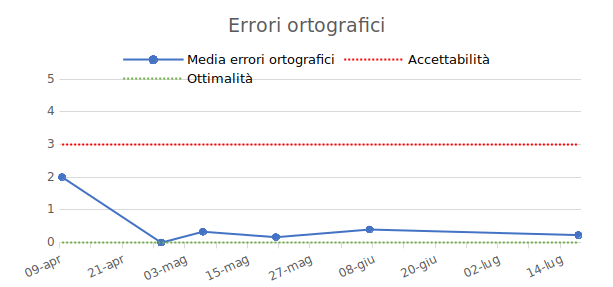
\includegraphics[scale=0.75]{img/Grafici/Errori_orto.png}
	\caption{Media degli errori ortografici.}
	\label{fig:Errori_orto}
\end{figure}

Il grafico evidenzia che la il numero medio di errori ortografici, è rimasto sempre entro i limiti di accettabilità.

\subsubsection{Errori concettuali}

Durante l'ultima verifica, sono stati rilevati all'interno dei vari documenti alcuni errori concettuali, il cui numero è specificato nel seguente grafico:

\begin{figure}[h!]
	\centering
	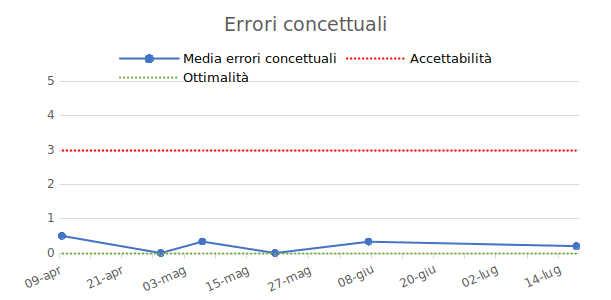
\includegraphics[scale=0.75]{img/Grafici/Errori_conce.png}
	\caption{Media degli errori concettuali}
	\label{fig:Errori_conce}
\end{figure}

Il grafico evidenzia che la il numero medio di errori concettuali è rimasto sempre entro i limiti di accettabilità.

\newpage
\subsubsection{Errori di forma}

Durante l'ultima verifica, sono stati rilevati all'interno dei vari documenti alcuni errori forma, il cui numero è specificato nel seguente grafico:

\begin{figure}[h!]
	\centering
	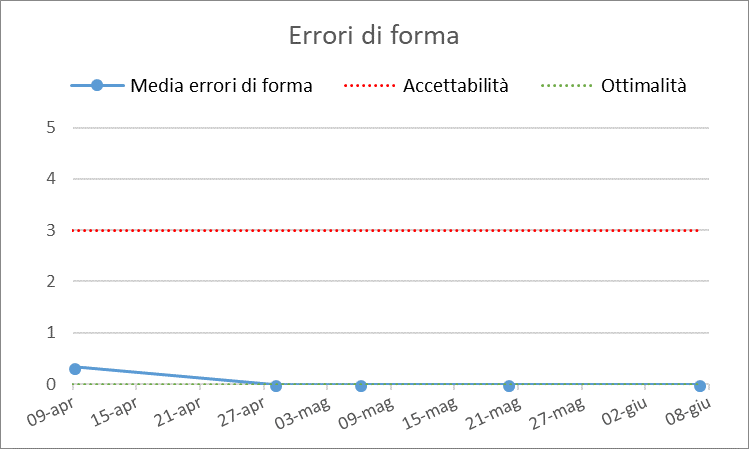
\includegraphics[scale=0.75]{img/Grafici/Errori_forma.png}
	\caption{Media degli errori di forma.}
	\label{fig:Errori_forma}
\end{figure}

Il grafico evidenzia che la il numero medio di errori di forma è rimasto sempre entro i limiti di accettabilità.

\subsubsection{Indice Gulpease}

Tutti i documenti consegnati sono stati sottoposti al calcolo dell'Indice Gulpease per valutarne il grado di leggibilità, il quale è riportato nel seguente grafico:

\begin{figure}[h!]
	\centering
	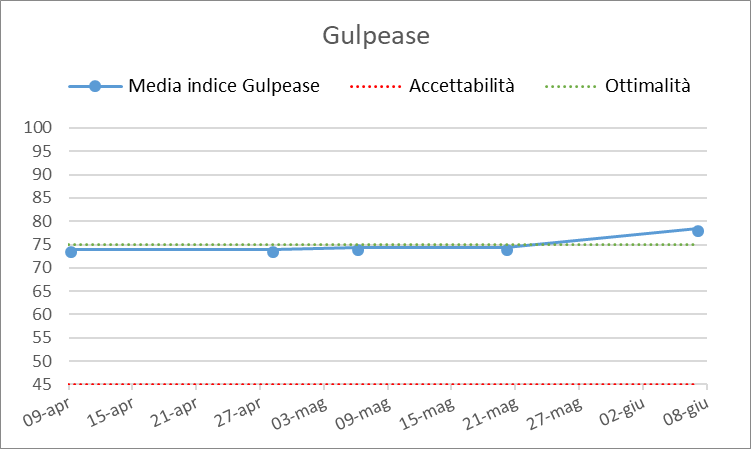
\includegraphics[scale=0.75]{img/Grafici/Gulpease.png}
	\caption{Media dell'indice di Gulpease; più il valore è alto, più ci si avvicina all'ottimalità.}
	\label{fig:Gulpease}
\end{figure}

Il grafico evidenzia che la il valore medio del calcolo dell'indice di gulpease è rimasto sempre entro i limiti di accettabilità, quasi raggiungendo l'ottimalità.
\subsection{Verifica dei processi}
\subsubsection{Schedule Variance}
Nel seguente grafico vengono riportati i valori ottenuti calcolando la Schedule Variance sui tempi di stesura dei documenti, progettazione e codifica del prodotto software rispetto ai tempi prefissati nel \PdP{}:

\begin{figure}[h!]
	\centering
	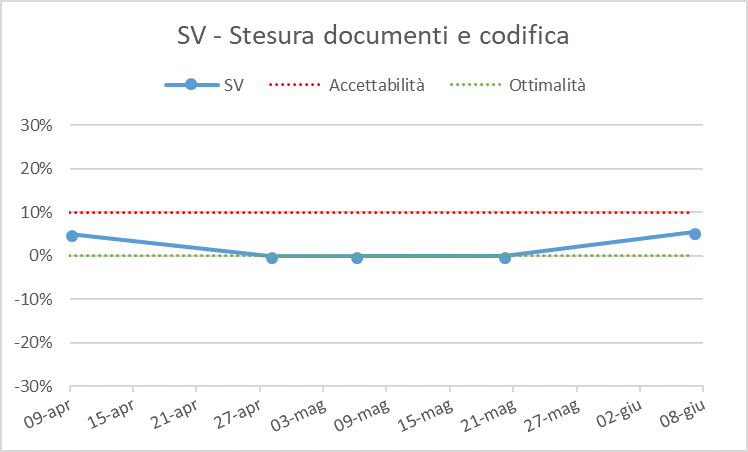
\includegraphics[scale=0.75]{img/Grafici/SV.png}
	\caption{Schedule Variance sui processi di stesura dei documenti, progettazione e codifica.}
	\label{fig:SV-Documenti}
\end{figure}

Il grafico evidenzia come il team sia riuscito a portare a termine i propri compiti sempre in tempo, oscillando tra accettabilità e ottimalità.

\subsubsection{Cost Variance}
Il calcolo della Cost Variance sui processi di documentazione e codifica ha portato il seguente risultato: 

\begin{figure}[h!]
	\centering
	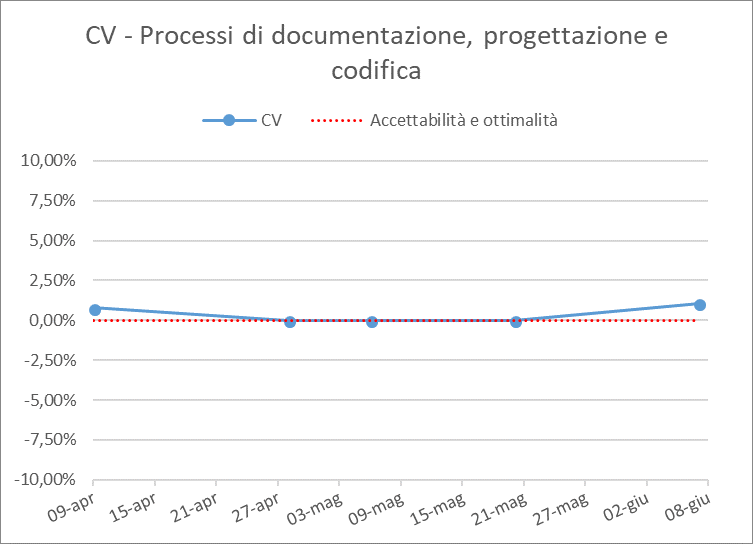
\includegraphics[scale=0.75]{img/Grafici/CV-cod_e_doc.png}
	\caption{Cost Variance per il processo di documentazione e codifica.}
	\label{fig:CV-Documenti}
\end{figure}

Il grafico evidenzia che la cost variance calcolata sui processi di documentazione e codifica è rimasta sempre entro i limiti di ottimalità.

\newpage
Di seguito vengono mostrati i risultati calcolati negli ultimi due periodi trascorsi, in cui si è iniziato ad utilizzare le metriche riguardanti la qualità del codice prodotto, al fine di evidenziare le differenze tra il codice della PoC e quello attuale.

\subsubsection{Schedule Variance - processo di verifica}
Nel seguente grafico vengono riportati i valori ottenuti calcolando la Schedule Variance sui tempi di verifica dei documenti e del prodotto software rispetto ai tempi prefissati nel \PdP{}:

\begin{figure}[h!]
	\centering
	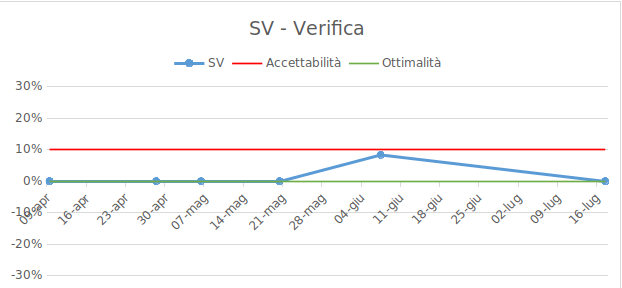
\includegraphics[scale=0.75]{img/Grafici/SV-Verifica.png}
	\caption{Schedule Variance per il processo di verifica.}
	\label{fig:SV-VerDocumenti}
\end{figure}

Il grafico evidenzia che la schedule variance calcolata sul processo di verifica della documentazione è rimasta sempre entro i limiti di accettabilità.


\subsubsection{Cost Variance - verifica}
Il calcolo della Cost Variance sul processo di verifica ha portato il seguente risultato: 

\begin{figure}[h!]
	\centering
	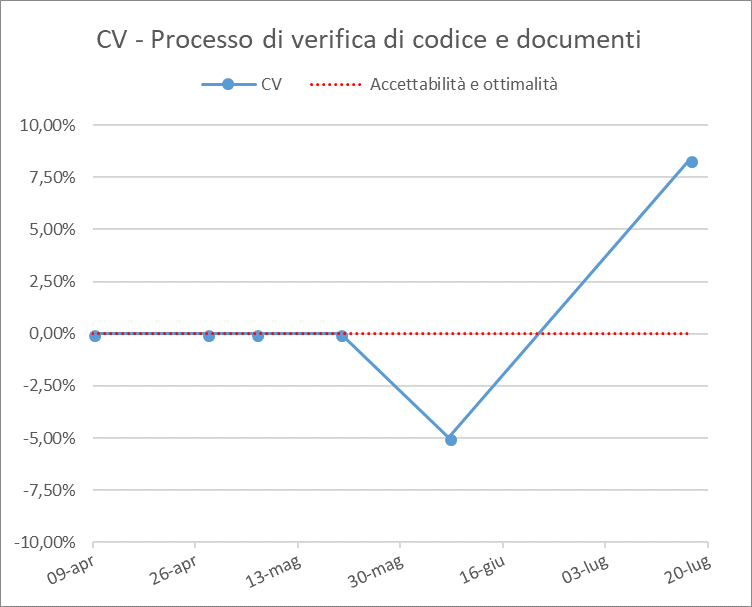
\includegraphics[scale=0.75]{img/Grafici/CV-verifica.png}
	\caption{Cost Variance per il processo di verifica.}
	\label{fig:CV-VerDocumenti}
\end{figure}

Il grafico evidenzia che la cost variance calcolata sul processo di verifica, è rimasta sempre entro i limiti di accettabilità e ottimalità, tranne nell'ultimo periodo in cui l'implementazione e l'esecuzione dei test ha richiesto alcune ore aggiuntive impiegate dai verificatori.

\newpage

\subsubsection{Rischi non preventivati}

Tale metrica è stata aggiunta dopo le prime fasi del progetto, dato che il team si è reso conto di aver bisogno di una maggior attenzione ai rischi, per essere sicuro di gestirli correttamente nel momento della loro manifestazione.

\begin{figure}[h!]
	\centering
	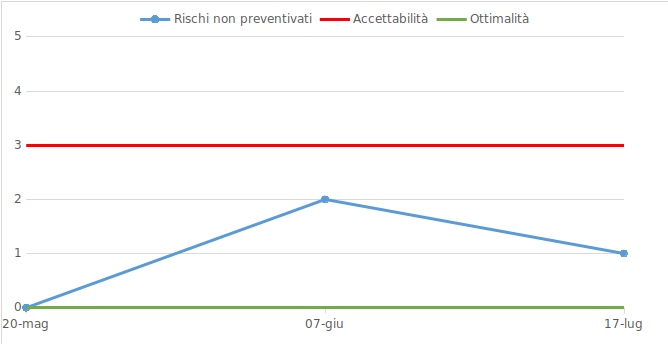
\includegraphics[scale=0.75]{img/Grafici/Rischi.png}
	\caption{Rischi non preventivati negli ultimi due periodi.}
	\label{fig:Rischi}
\end{figure}

Il grafico evidenzia che sono stati riscontrati alcuni rischi non preventivati, la cui causa è la scarsa conoscenza pregressa da parte del team delle tecnologie utilizzate, dato che in questo periodo si è cominciato ad utilizzarle più nel dettaglio.

\subsubsection{Complessità ciclomatica}

\begin{figure}[h!]
	\centering
	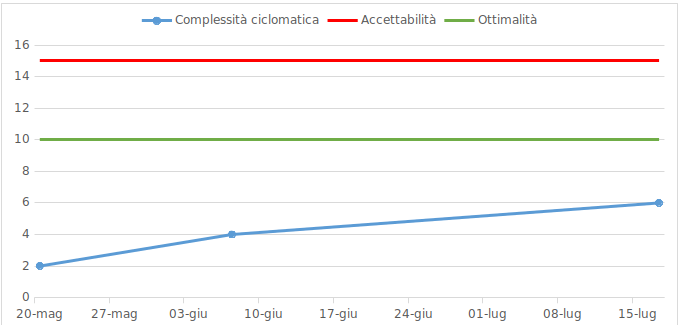
\includegraphics[scale=0.75]{img/Grafici/ciclomatica.png}
	\caption{Complessità ciclomatica.}
	\label{fig:Ciclomatica}
\end{figure}

Il grafico evidenzia come la maggior complessità delle funzionalità offerte dal prodotto durante lo sviluppo si riflette in una maggior complessità del codice stesso.

\subsubsection{SFIN - Structural fan in}

Essendo questo risultato una media complessiva calcolata sulle classi presenti nel codice dell'intero progetto, si è ritenuto riportarla singolarmente, senza calcolare anche la SFOUT - Structural fan out, per evitare la ripetizione di un risultato identico.

\begin{figure}[h!]
	\centering
	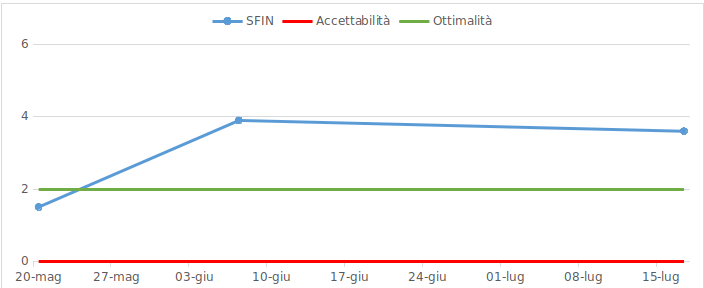
\includegraphics[scale=0.75]{img/Grafici/SFIN.png}
	\caption{Structural fan in, più il valore è alto, meglio è.}
	\label{fig:SFIN}
\end{figure}

Nonostante inizialmente si è rimasti sotto l'ottimalità, con il crescere del prodotto si è arrivati a superare di gran lunga la soglia di ottimalità, il che indica un alto riuso del codice. 

\subsubsection{CxSLOC - Commenti per linee di codice}

\begin{figure}[h!]
	\centering
	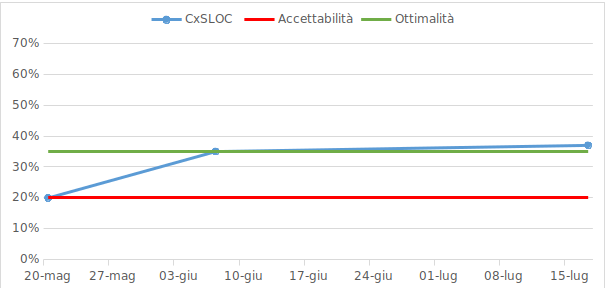
\includegraphics[scale=0.75]{img/Grafici/CxSLOC.png}
	\caption{Commenti per linee di codice, un valore alto è positivo.}
	\label{fig:CxSLOC}
\end{figure}

Il grafico evidenzia come il team si sia impegnato a fornire un codice quanto più capibile possibile, aumentando di molto la percentuale di commenti rispetto alla versione iniziale del prodotto.

\newpage

\subsubsection{Parametri per metodo}

\begin{figure}[h!]
	\centering
	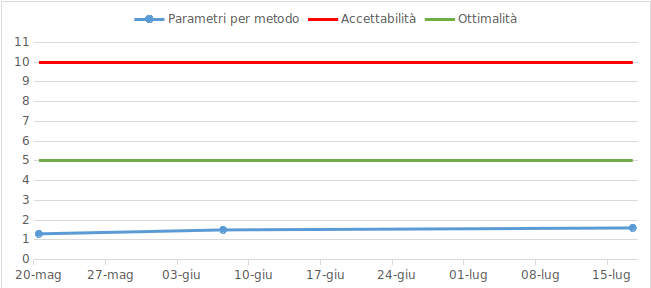
\includegraphics[scale=0.75]{img/Grafici/param_metodo.png}
	\caption{Numero di parametri per metodo, un numero basso indica meno complessità.}
	\label{fig:param_metodo}
\end{figure}

Mediamente, i metodi scritti dal team sono risultati poco complessi sotto questo punto di vista, con un numero di parametri ben oltre la soglia di ottimalità.

\subsubsection{Linee di codice per metodo}

\begin{figure}[h!]
	\centering
	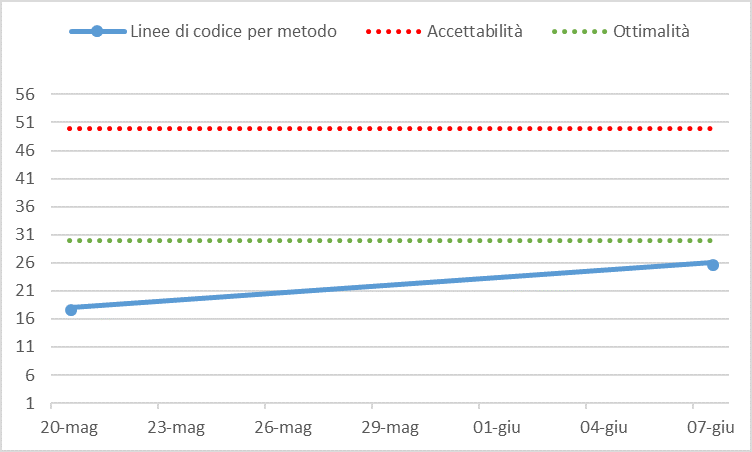
\includegraphics[scale=0.75]{img/Grafici/Linee_metodo.png}
	\caption{Linee di codice per metodo, un numero basso indica meno complessità.}
\end{figure}

Mediamente, i metodi scritti dal team sono risultati non troppo complessi sotto questo punto di vista, con un numero di righe ottimali.

\newpage

\subsubsection{ROF - Requisiti obbligatori soddisfatti}

\begin{figure}[h!]
	\centering
	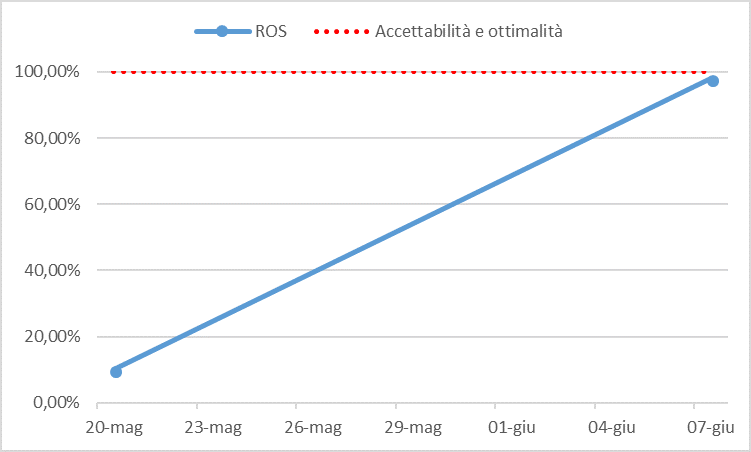
\includegraphics[scale=0.75]{img/Grafici/ROS.png}
	\caption{Requisiti obbligatori soddisfatti.}
\end{figure}

Il grafico mostra come nonostante la prima bozza del prodotto coprisse una percentuale esigua di requisiti, il team è risuscito a soddisfarli quasi tutti con la versione attuale del prodotto.


\subsubsection{ROFS - Requisiti obbligatori e facoltativi soddisfatti}

\begin{figure}[h!]
	\centering
	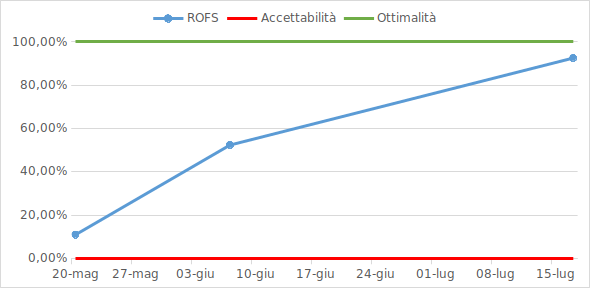
\includegraphics[scale=0.75]{img/Grafici/ROFS.png}
	\caption{Requisiti obbligatori e facoltativi soddisfatti.}
\end{figure}

Il grafico mostra come anche una buona parte dei requisiti facoltativi sono stati soddisfatti.

\newpage

\subsubsection{Successo dei test}

\begin{figure}[h!]
	\centering
	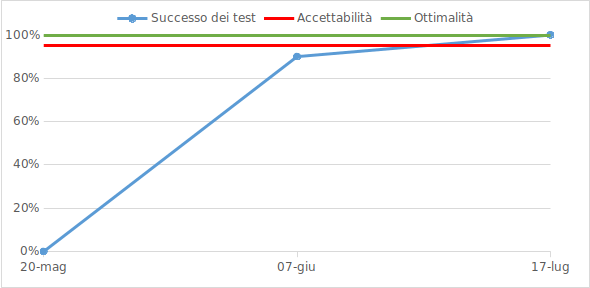
\includegraphics[scale=0.75]{img/Grafici/successo_test.png}
	\caption{Percentuale di successo dei test.}
\end{figure}

Il grafico mostra che una grossa percentuale dei test finora sviluppati hanno esito positivo, tuttavia tale risultato rimane ancora sotto la soglia di accettabilità.



